\chapter{Discussion, Conclusion and Future Work}\label{chapter:discussion}

In this chapter, we discuss the results of the experiments conducted in Chapter \ref{chapter:results}. We will discuss the effect of different parameters on the performance of the models, 
and how they relate to the original goals of this thesis. We then conclude with a summary of the findings and suggest future work that can be done.

\section{Effect of Phoneme Count}

\begin{figure}[H]  
    \centering
    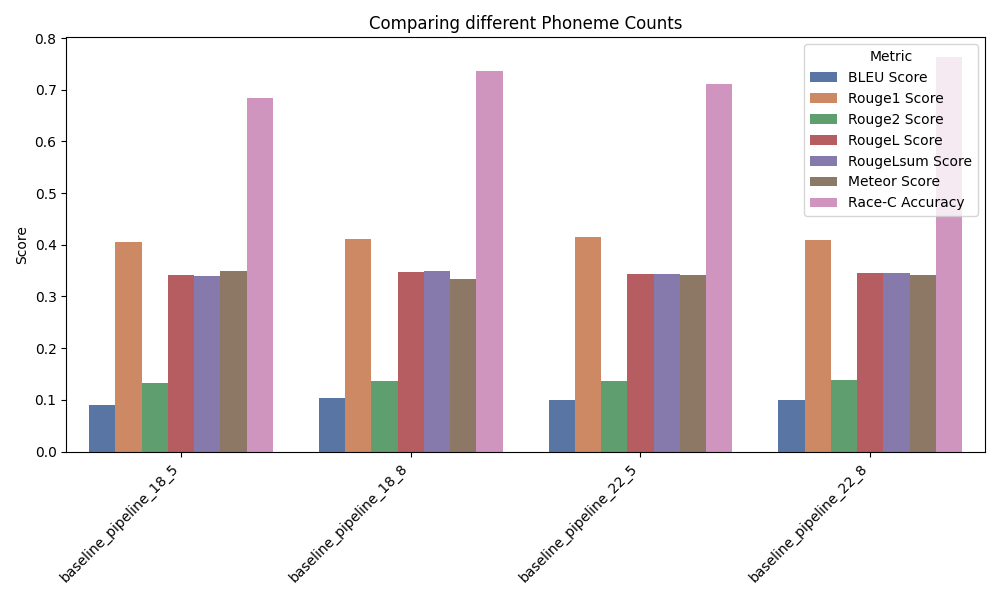
\includegraphics[width=0.7\linewidth]{figures/results/1_effect_of_phoneme_count.png}
    \caption{Comparing the Effects of different phoneme counts}
    \label{fig:compare-phoneme-count}
\end{figure}

As we can see in Figure \ref{fig:compare-phoneme-count}, the phoneme count does not seem to have a significant effect on the translation scores
or the Race-C scores. This being the case, we can conclude that we can simplify a language by reducing the phoneme count without affecting the 
ability of the language to convey meaning. 

\section{Effect of Phonotactics}

\begin{figure}[H]  
    \centering
    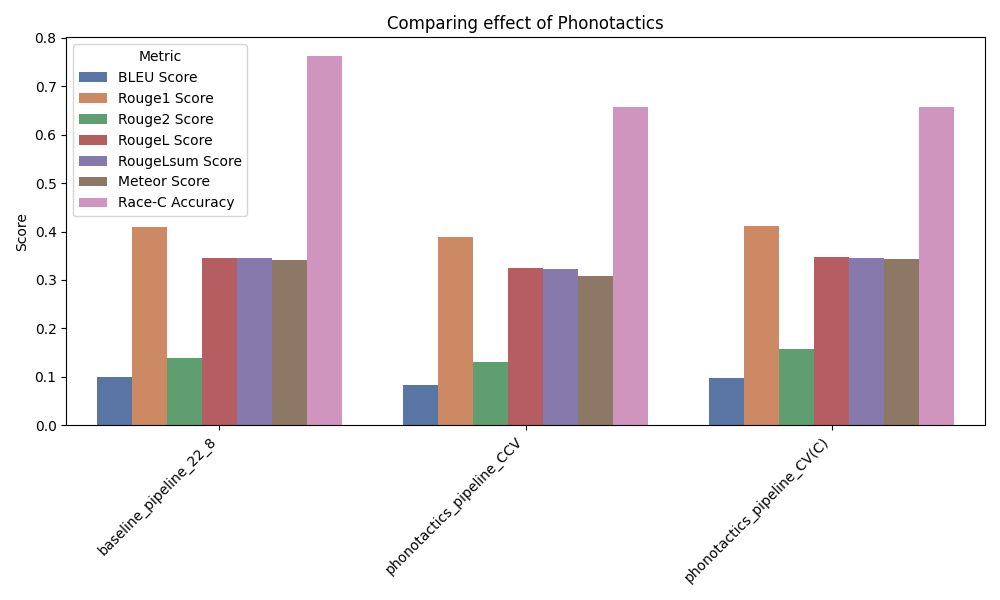
\includegraphics[width=0.7\linewidth]{figures/results/1_effect_of_phonotactics.png}
    \caption{Comparing the Effects of phonotactics}
    \label{fig:compare-phonotactics}
\end{figure}

Figure \ref{fig:compare-phonotactics} shows the effect of phonotactics on the translation scores and the Race-C scores. Again, we can see that
the phonotactics do not seem to have a significant effect either of the metrics. We can therefore conclude that we can simplify a language by 
using simplifed phonotactic rules without affecting the ability of the language to convey meaning.

\section{Effect of Grammar Rules}

\begin{figure}[H]  
    \centering
    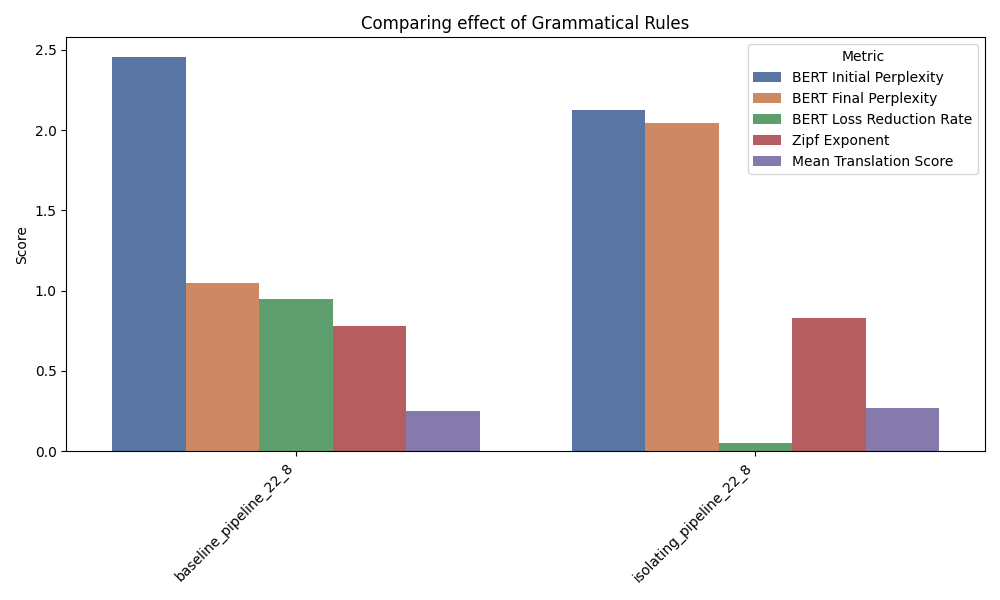
\includegraphics[width=0.7\linewidth]{figures/results/1_effect_of_grammar.png}
    \caption{Comparing different Grammatical Rules}
    \label{fig:compare-grammar}
\end{figure}



\section{Effect of Vocabulary Generation method}

Figure \ref{fig:compare-vocab-gen-types} shows the effect of different vocabulary generation methods against our metrics.

\section{Effect of Language Model Temperature}